\section{Rebuilding the benchmark}

% ------------------------------------------------------------------------------
\begin{frame}{Layer \ding{172}: one entry per good unit, no template}
  \centering
  \begin{tikzpicture}[node distance=4mm and 10mm,
      codebox/.style={box, align=left, font=\ttfamily\scriptsize, inner sep=3pt}]
    % original good
    \node[codebox, draw=WarnDraw, fill=WarnFill] (orig) {%
      \textcolor{OIvermil}{\textbf{static void}} G2B()\ \{ ALLOCA \}\\
      \textcolor{OIvermil}{\textbf{static void}} B2G()\ \{ malloc \dots\ free \}\\
      void good()\ \{ G2B(); B2G(); \}};
    \node[lbl, above=1mm of orig] {original good unit};
    % layer-1 good units (one per group)
    \node[codebox, draw=DataDraw, fill=DataFill, right=6mm of orig, yshift=7mm] (g2b) {%
      {\sffamily\bfseries G2B:}\ void sym\_0()\ \{ ALLOCA \dots\ \}};
    \node[codebox, draw=DataDraw, fill=DataFill, below=4mm of g2b.south west, anchor=north west] (b2g) {%
      {\sffamily\bfseries B2G:}\ void sym\_0()\ \{ malloc \dots\ free \}};
    \node[lbl] at ($(g2b.north)+(0,3mm)$) {layer \ding{172}: two good units};
    \draw[arr] (orig.east) -- (g2b.west);
    \draw[arr] (orig.east) -- (b2g.west);
    \node[lbl, text=Ink, below=7mm of orig] (rules) {pick \textbf{one} good entry per group\quad
      $\cdot$\quad drop the wrapper\quad$\cdot$\quad strip \code{static}};
  \end{tikzpicture}
  \vspace{4pt}
  \begin{itemize}
    \item Bad units unchanged; good units now look like bad units (same shape, same length)
    \item G2B / B2G split $\approx$ 50/50 inside every flow category (e.g.\ 02--22: 323 / 323)
    \item G2B good has \emph{no} \code{free} (stack memory): grep's rule is now wrong there
  \end{itemize}
\end{frame}

% ------------------------------------------------------------------------------
\begin{frame}{Shortcut probes: before vs after debiasing}
  \begin{columns}[c]
    \begin{column}{0.60\textwidth}
      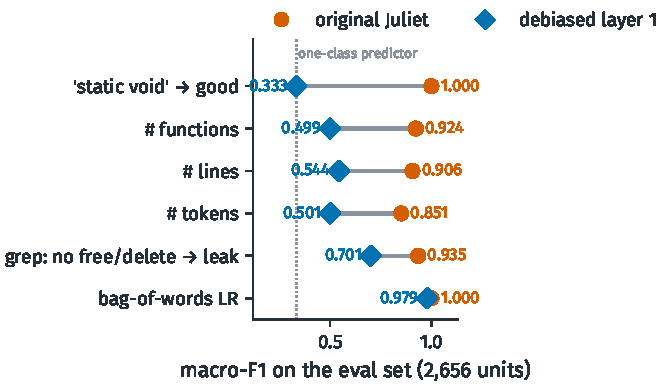
\includegraphics[width=\linewidth]{figures/probes.pdf}
    \end{column}
    \begin{column}{0.38\textwidth}
      \begin{itemize}
        \item Format probes fall to chance (\code{static void}: 1.000 $\to$ 0.333)
        \item grep 0.935 $\to$ 0.701: it fails on G2B good units
        \item Bag-of-words stays at 0.979: its cues (\code{free}, \code{delete}, \code{ALLOCA}) are about the task itself
      \end{itemize}
    \end{column}
  \end{columns}
  \vfill
  {\scriptsize Probes fitted on dev, scored on eval; acceptance: every format probe $\le 0.60$ (all pass).}
\end{frame}

% ------------------------------------------------------------------------------
\begin{frame}{Are the labels still right? Compile and run every unit}
  \begin{columns}[T]
    \begin{column}{0.50\textwidth}
      \begin{itemize}
        \item gcc and clang compile \textbf{3,316 / 3,316} units (both layers)
        \item ASan/LSan: \textbf{1,658 / 1,658} good units leak-free
        \item Labels are never changed; disagreements are explained, not relabelled
      \end{itemize}
    \end{column}
    \begin{column}{0.47\textwidth}
      {\small LSan reports a leak on the \emph{bad} unit\\[2pt]
      \begin{tabular}{@{}lr@{}}
        \toprule
        Mechanism & detected \\
        \midrule
        C \code{malloc}-family & 914 / 960 \\
        C++ \code{new} & 558 / 588 \\
        destructor & 2 / 2 \\
        \code{realloc} failure & \alert{0 / 108} \\
        \bottomrule
      \end{tabular}}
    \end{column}
  \end{columns}
  \vfill
  {\small Dynamic tools are a \textbf{reference line}, not an upper bound: misses need a failing \code{realloc},
  memory still reachable from a global at exit, or a random branch (appendix).}
\end{frame}

% ------------------------------------------------------------------------------
\begin{frame}[fragile]{Three evaluation layers}
  \centering
  \begin{tikzpicture}[node distance=5mm and 9mm]
    \node[hero, minimum width=30mm, minimum height=11mm] (l1) {\textbf{\ding{172} Debiased main}\\{\scriptsize 3,316 units}};
    \node[data, right=14mm of l1, yshift=7mm, minimum width=40mm] (l2) {\textbf{\ding{173} Natural hard subset}\\{\scriptsize bad units that do contain a free}};
    \node[warn, right=14mm of l1, yshift=-7mm, minimum width=40mm] (l3) {\textbf{\ding{174} Stress test + placebo}\\{\scriptsize add frees that never run}};
    \draw[arr] (l1.east) -- node[lbl, above, sloped] {filter} (l2.west);
    \draw[arr] (l1.east) -- node[lbl, below, sloped] {transform} (l3.west);
  \end{tikzpicture}
  \vspace{2pt}
  \begin{columns}[T]
    \begin{column}{0.48\textwidth}
      {\small \textbf{bad} + dead free $\Rightarrow$ still \alert{leak}}
\begin{lstlisting}[style=unit]
static const int sym_7 = 5;
data = (char *)malloc(100);
(*\hlc{if (sym\_7 != 5) \{ free(data); \}}*)
\end{lstlisting}
    \end{column}
    \begin{column}{0.48\textwidth}
      {\small \textbf{good}: real free, always-true guard}
\begin{lstlisting}[style=unit]
(*\hlc{if (sym\_7 == 5) \{ free(data); \}}*)
\end{lstlisting}
      {\small \textbf{placebo}: same guard, no free}
\begin{lstlisting}[style=unit]
if (sym_7 != 5) { printLine("..."); }
\end{lstlisting}
    \end{column}
  \end{columns}
  \vfill
  {\scriptsize All 3,316 units; guards are decidable inside one file; both labels get guarded frees (grep: macro-F1 0.333 on \ding{174}).\\ Every transformed unit compiles (gcc, clang) and is re-checked with ASan/LSan.\par}
\end{frame}

% ------------------------------------------------------------------------------
\begin{frame}{Split by flow variant, not by family}
  \centering
  \begin{tikzpicture}[x=0.071mm, y=1mm]
    % widths proportional to groups: dev 330, fold0 472, fold1 424, fold2 432 (total 1,658)
    \foreach \x/\w/\c/\name/\sub in {0/330/NeutFill/dev/9 variants, 330/472/HeroFill/fold 0/15 variants,
        802/424/HeroFill/fold 1/12 variants, 1226/432/HeroFill/fold 2/12 variants}{
      \fill[\c, draw=NeutDraw, line width=0.5pt] (\x,0) rectangle ++(\w,9);
      \node[font=\small] at (\x+\w/2,5.6) {\textbf{\name}};
      \node[font=\scriptsize, text=NeutDraw] at (\x+\w/2,2.6) {\sub};
    }
    \draw[decorate, decoration={brace, amplitude=4pt, mirror}, NeutDraw] (0,-1) -- (330,-1)
      node[midway, below=4pt, lbl] {330 groups: prompts, thresholds,\\ checkpoints (never reported)};
    \draw[decorate, decoration={brace, amplitude=4pt, mirror}, HeroDraw] (330,-1) -- (1658,-1)
      node[midway, below=4pt, lbl, text=HeroDraw] {eval: 39 variants, 1,328 groups = 2,656 units};
  \end{tikzpicture}
  \vspace{2pt}
  \begin{itemize}
    \item Families differ mostly by data type (\code{char\_malloc} vs \code{int\_malloc}): a family split leaks structure
    \item Flow-variant split $\Rightarrow$ test on \textbf{unseen program structure}
    \item Fine-tuning: train on two folds, predict the third; dev only selects epoch and threshold
    \item Metrics: P / R / F1 (leak = positive) and macro-F1; family-bootstrap CI; McNemar + Holm
  \end{itemize}
\end{frame}
